% This LaTeX was auto-generated from MATLAB code.
% To make changes, update the MATLAB code and export to LaTeX again.

\documentclass{article}

\usepackage[utf8]{inputenc}
\usepackage[T1]{fontenc}
\usepackage{lmodern}
\usepackage{graphicx}
\usepackage{color}
\usepackage{hyperref}
\usepackage{amsmath}
\usepackage{amsfonts}
\usepackage{epstopdf}
\usepackage[table]{xcolor}
\usepackage{matlab}

\sloppy
\epstopdfsetup{outdir=./}
\graphicspath{ {./RUNME_images/} }

\matlabhastoc

\begin{document}

\label{T_40EA8FCF}
\matlabtitle{The impact of Cognitive Tasks on Network Properties after abrupt awakening}

\matlabtableofcontents{Table of Contents}

\label{H_0F12C076}
\matlabheading{Summary}

\begin{par}
\begin{flushleft}
Interestingly the network appears to change in opposite ways accross multiple dimensions
\end{flushleft}
\end{par}

\begin{itemize}
\setlength{\itemsep}{-1ex}
   \item{\begin{flushleft} the frequency band that changes - upper or lower \end{flushleft}}
   \item{\begin{flushleft} the onset time of the change in the network - either network property is immediately effected or delayed \end{flushleft}}
   \item{\begin{flushleft} the duration of change in the network- either for a single test bout, or extended \end{flushleft}}
\end{itemize}

\begin{par}
\begin{flushleft}
Notice that during the PV Task, the DELTA network is impacted immediately and temporaly after waking. Namely, clustering increases and path length decreases at time 1, but recovers quickly by time 2.
\end{flushleft}
\end{par}

\begin{par}
\begin{flushleft}
In contras during the Math Task, it is the BETA network that changes, and this change is not immediate and does not appear to recover. Namely, clustering increases and path length decreases during the seccond, third and fourth test bout.
\end{flushleft}
\end{par}


\label{H_44835ED9}
\matlabheading{Get Data Set}

\begin{matlabcode}
clear;
DFM = dfmaster();  
\end{matlabcode}
\begin{matlaboutput}
##########
Getting GPSD during PVT Task. . . . . . . . . . . . 
	DONE

##########
Getting Network Props during PVT : . . . . . . . . . . . . 
	done
##########
Getting GPSD during KDT Task. . . . . . . . . . . 
	DONE

##########
Getting Network Props during KDT : . . . . . . . . . . . 
	done
##########
Getting GPSD during MATH Task. . . . . . . . . . . . 
	DONE

##########
Getting Network Props during MATH : . . . . . . . . . . . . 
	done
##########
Getting GPSD during GONOGO Task. . . . . . . . . . . . 
	DONE

##########
Getting Network Props during GONOGO : . . . . . . . . . . . . 
	done
\end{matlaboutput}
\begin{matlabcode}
clearvars -except DFM   
close all
\end{matlabcode}


\label{H_BA23F496}
\matlabheading{CLUSTERING and PATH LENGTH of LOW FREQUENCIES}

\label{H_7A8D528B}
\matlabheadingtwo{Low frequency components change only while engaging in PVT task. }

\begin{itemize}
\setlength{\itemsep}{-1ex}
   \item{\begin{flushleft} Notice that during the PV Task, the DELTA network is impacted immediately and temporaly after waking.  \end{flushleft}}
   \item{\begin{flushleft} Namely, clustering increases and path length decreases at time 1, but recovers quickly by time 2. \end{flushleft}}
   \item{\begin{flushleft} further more, the DELTA network remains unnaffected while engagin in the math task \end{flushleft}}
\end{itemize}

\begin{matlabcode}
figanz_cogtestcmp(DFM, 'PVT', 'Math', 'clust', 'delta', 'control')
exportgraphics(gcf,'fig_clust_pvt_vs_math_beta_cntl.png','Resolution',100)
\end{matlabcode}
\begin{center}
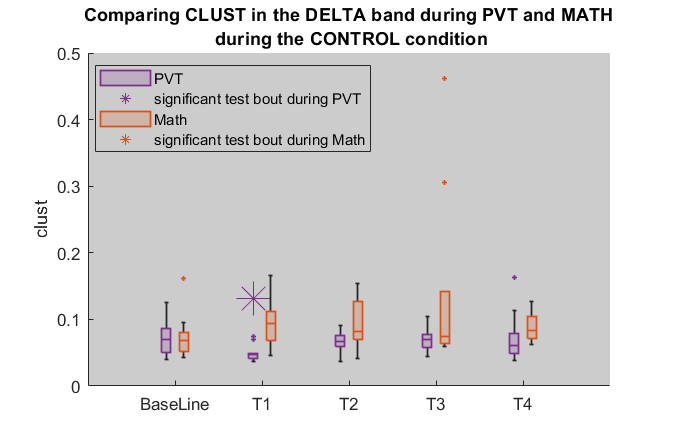
\includegraphics[width=\maxwidth{54.08931259407928em}]{figure_0.png}
\end{center}
\begin{matlabcode}
figanz_cogtestcmp(DFM, 'PVT', 'Math', 'pathl', 'delta', 'control')
exportgraphics(gcf,'fig_clust_pvt_vs_math_delta_cntl.png','Resolution',100)
\end{matlabcode}
\begin{center}
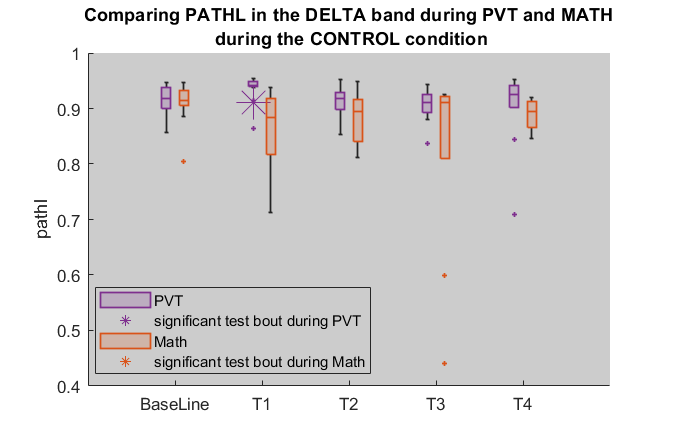
\includegraphics[width=\maxwidth{54.08931259407928em}]{figure_1.png}
\end{center}


\label{H_ACDBA229}
\matlabheading{CLUSTERING and PATH LENGTH of HIGH FREQUENCIES}

\label{H_47648F53}
\matlabheadingtwo{High frequency networl components change only while engaging in Math task. }

\begin{itemize}
\setlength{\itemsep}{-1ex}
   \item{\begin{flushleft} Notice that during the Math Task, it is the BETA network that changes \end{flushleft}}
   \item{\begin{flushleft} Namely, clustering increases and path length decreases  \end{flushleft}}
   \item{\begin{flushleft} Note that unlike the lower frequency, this change is not immediate nor does it recover by the fourth test bout.  \end{flushleft}}
   \item{\begin{flushleft} Further more, these effects are only visible while engaging in the MATH task \end{flushleft}}
\end{itemize}

\label{H_1ABFDAE1}
\matlabheadingthree{Compare the Low and hight fequency componenets}

\begin{par}
\hfill \break
\end{par}

\begin{matlabcode}
figanz_cogtestcmp(DFM, 'PVT', 'Math', 'clust', 'beta', 'control')
exportgraphics(gcf,'fig_pathl_pvt_vs_math_beta_cntl.png','Resolution',100)
\end{matlabcode}
\begin{center}
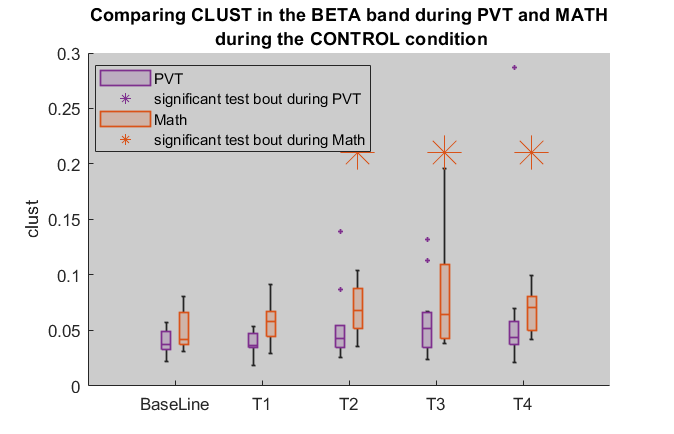
\includegraphics[width=\maxwidth{54.08931259407928em}]{figure_2.png}
\end{center}
\begin{matlabcode}

figanz_cogtestcmp(DFM, 'PVT', 'Math', 'pathl', 'beta', 'control')
exportgraphics(gcf,'fig_pathl_pvt_vs_math_beta_cntl.png','Resolution',100)
\end{matlabcode}
\begin{center}
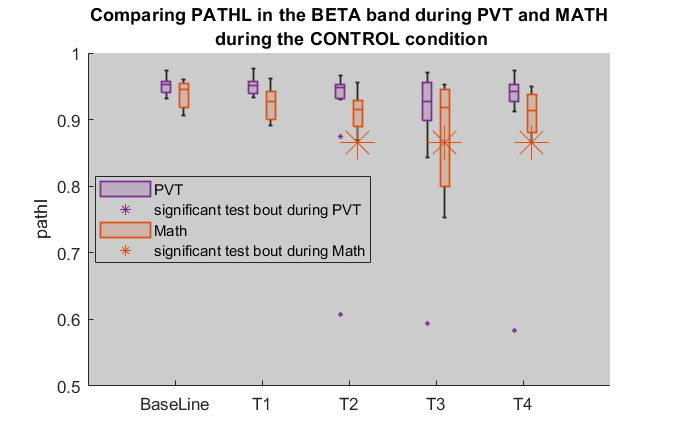
\includegraphics[width=\maxwidth{54.08931259407928em}]{figure_3.png}
\end{center}


\label{H_0A9FD214}
\matlabheading{Supplementary Figures: Original figure 1 analysis, but for all tasks. Ignore for now}

\begin{matlabcode}
fig1anz(DFM, 'gpsd')
exportgraphics(gcf,'fig_fig1Original_gpsd.png','Resolution',100)
\end{matlabcode}
\begin{center}
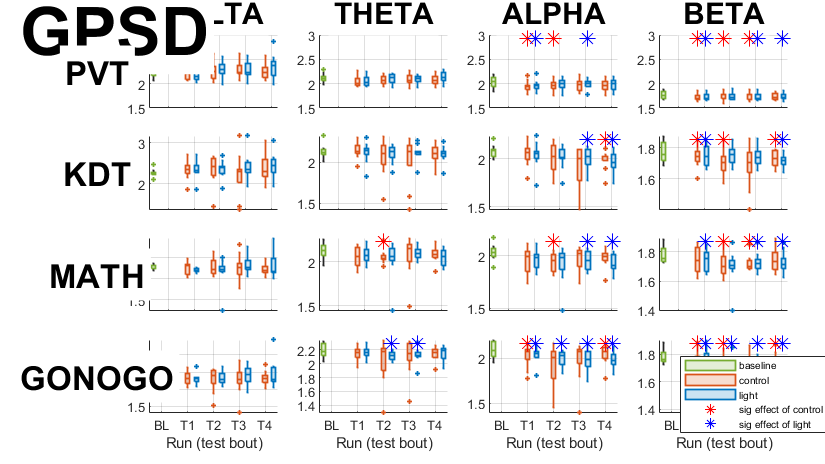
\includegraphics[width=\maxwidth{66.23181133968892em}]{figure_4.png}
\end{center}
\begin{matlabcode}

fig1anz(DFM, 'clust')
exportgraphics(gcf,'fig_fig1Original_clust.png','Resolution',100)
\end{matlabcode}
\begin{center}
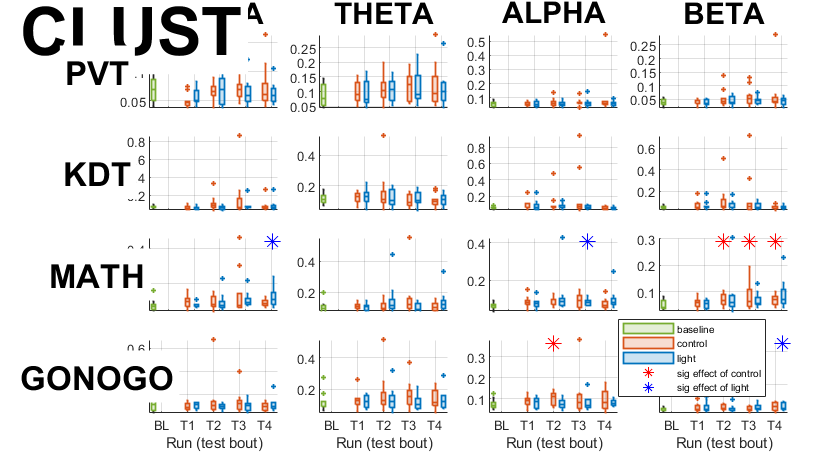
\includegraphics[width=\maxwidth{66.23181133968892em}]{figure_5.png}
\end{center}
\begin{matlabcode}

fig1anz(DFM, 'pathl')
exportgraphics(gcf,'fig_fig1Original_pathl.png','Resolution',100)
\end{matlabcode}
\begin{center}
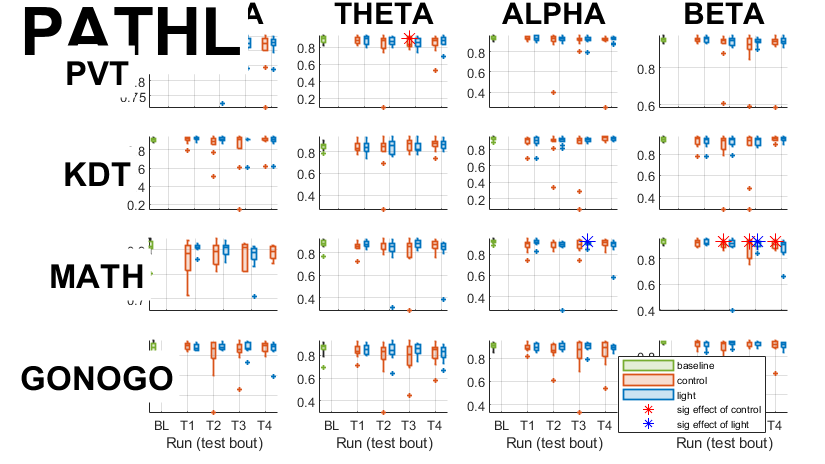
\includegraphics[width=\maxwidth{66.23181133968892em}]{figure_6.png}
\end{center}

\end{document}
